%----------------------------------------------------------------------------
\chapter{Overview of the framework}
%----------------------------------------------------------------------------

%%
%% Futásidejű dolgok és kódgenerálás is!
%%

This chapter provides an overview of the approach to runtime monitoring of cyber-physical systems, and describes the basic architecture of the implemented monitoring framework.

\section{Runtime verification approach}

An overview of the runtime monitoring approach is depicted in \autoref{fig:approach}. 
The left hand side illustrates the connections between \emph{design time artifacts}, while on the right hand side of the figure the \emph{running monitoring programs} are shown.

\begin{figure}[h]
	\begin{center}
		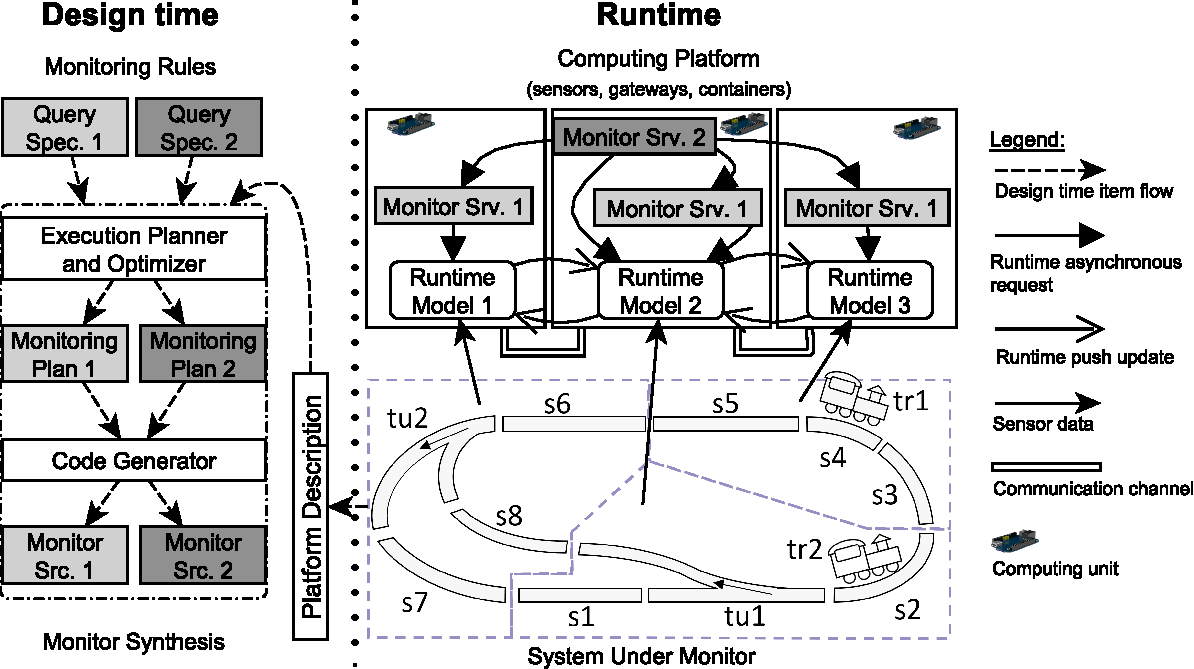
\includegraphics[width=\textwidth]{figures/fase-overview-crop.pdf}
		\caption{Approach to CPS monitoring}
		\label{fig:approach}
	\end{center}
\end{figure}

\subsection{Design time}

At first, the developer of the system must design the domain model of the CPS based on the structure of the target system.
From this domain model we generate the code that can be used to build up and maintain the live model of the system.

Then monitoring goals are defined as graph patterns. 
As patterns can refer to the meta model, it is a prerequisite for pattern definition. 
From these patterns we create monitoring plans. 
We use these plans to generate the source code of the monitoring components.

\subsection{Runtime}

At runtime, we rely on the generated monitor code and the generated model code. 
We create the nodes of the live model, create the references/edges between them and give the values of the attributes of the objects. 
With the physical world changing we update the objects to reflect the current state of the system. \todo{hivatkozasok a kesobbi reszekre, ahol ezekrol tobb szo esik}
On this model, we run the monitoring code to find matches for the patterns in the model. 
If a pattern match occurs, we find the model elements that conform the pattern, thus we can locate the problems in the model, representing the cyber-physical system.


\section{Framework architecture}

Users of the framework can design the domain models of the system using EMF Ecore modeling, while they can formulate monitoring goals as graph patterns using the declarative Viatra Query Language (VQL).
Based on these definitions, the framework generates the monitoring \cpp{} program code.
Besides the generated code, the framework provides and additional library to  along with additional libraries, that are used by the generated code. \todo{ez a mondat nincs befejezve}

\subsection{Code generation workflow}
A set of Eclipse plugins provide support to transform EMF Ecore models and VQL monitor definitions into \cpp code. \todo{nem biztos, hogy mindenhol megeri passzivot hasznalni}
These plugins are written in Xtend. \todo{ha a C++-t mas betutipussal irod, akkor szerintem erdemes a technologiakra, de legalabb a programnyelvekre konzisztensen ugyan azt a betutipust hasznalni}
\autoref{fig:workflow} shows the corresponding code generation workflow.

\begin{figure}[H]
	\begin{center}
		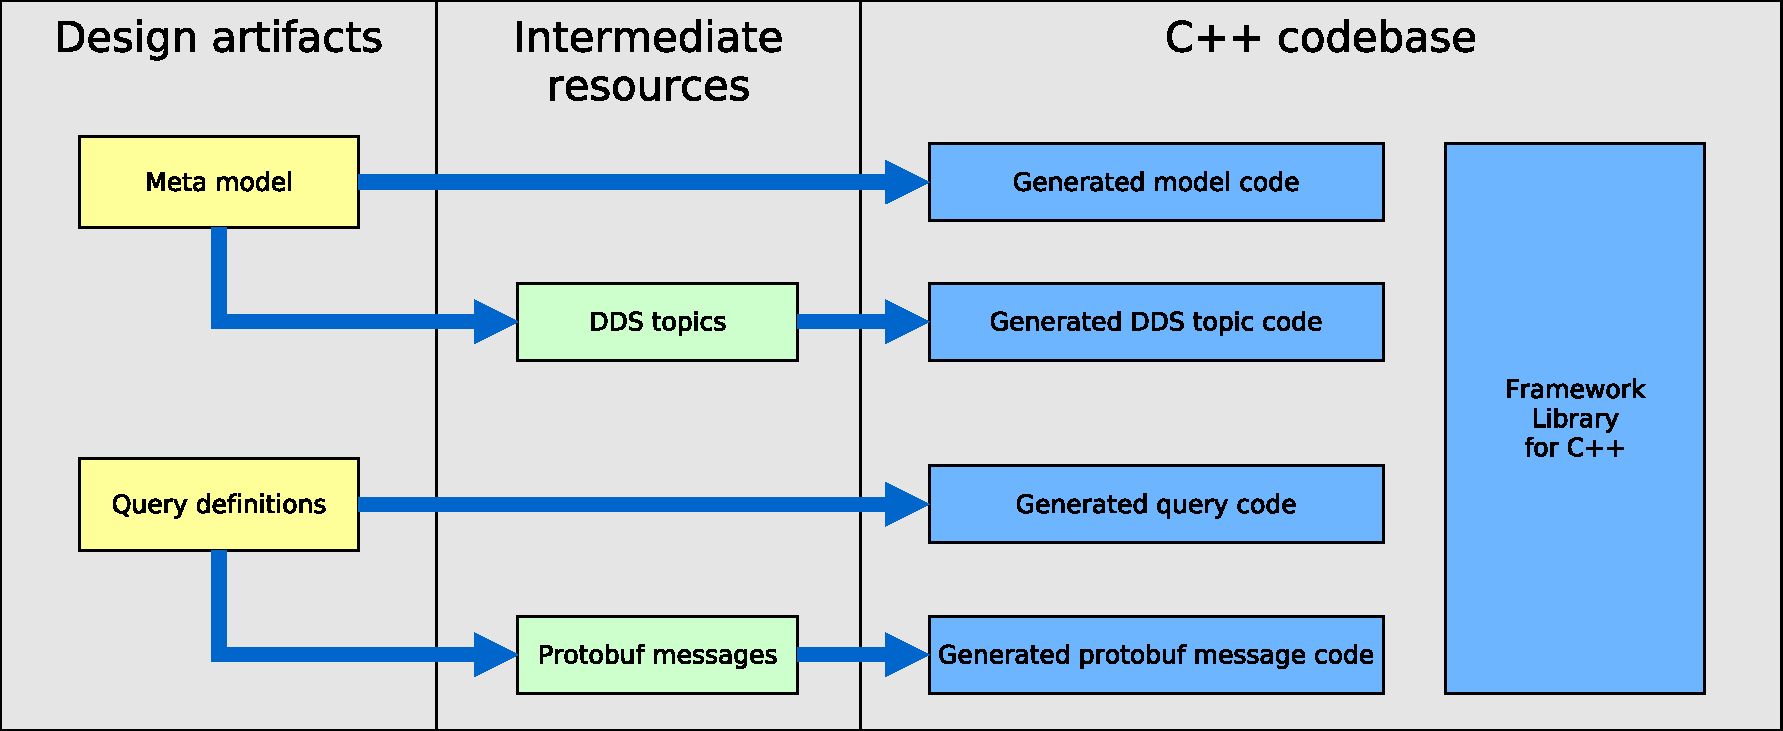
\includegraphics[width=\textwidth]{figures/workflow.pdf}
		\caption{Code generation input and output artifacts}
		\label{fig:workflow}
	\end{center}
\end{figure}

From the EMF metamodel we generate model code, which can be used to build up and maintain the live model. 
We also generate the corresponding DDS topics, as DDS is used to notify computation units about object creation/deletion and reference creation/deletion.

From the VQL files we parse the graph patterns and generate the code able to execute them.
Query execution depends on serialization/deserialization service provided by protobuf, so we also create the corresponding protobuf messages and compile them into \cpp{} code.
